\section{An EKF update using magnetometer measurements}

\subsection{Task 9}

For this segment, I have undertaken a fresh measurement of the magnetic parameters to recalibrate the magnetometer's offset.

The mean of mag -X is -4.973822 
, the covariance of mag -X is 0.303807  

The mean of mag -Y is 3.863684 
, the covariance of mag -Y is 0.311815 

The mean of mag -Z is -58.885704 
, the covariance of mag -Z is 0.340960 

From the measurement above we can see that it is far away from the result of the first chapter, so it is quite reasonable to do a new measurement.

The theory of EKF filter is the same with Accelerometer part, and the function  \texttt{mu\_m} is exactly modified from \texttt{mu\_g}.

\textcolor{red}{add the derivation here, modify from Acc part}


\subsection{Task 10}

\begin{figure}[H]
 \centering
 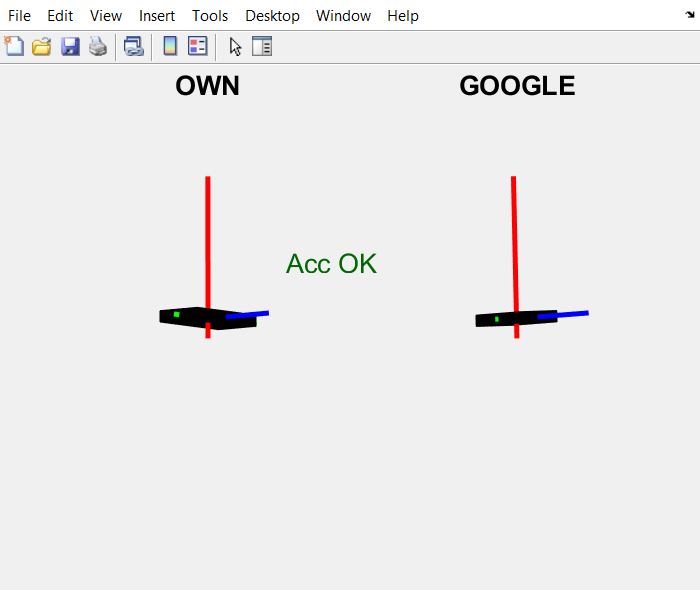
\includegraphics[width=0.6\textwidth]{images/magbegin.png}
 \caption{Begin state with magnetometer added}
 \label{magbegin}
\end{figure}

I gently move and rotate the phone. After the manipulation, the phone end up as a posture with an certain offset with the real google one. But after I place the phone on the table and wait it for sometime, I can abserve that the posture estimate of the phone slowly converge to the real value, which is not expressed in previous parts, and this phenomenon shows the magnetometer improved the estimate accuracy.

\begin{figure}[H]
 \centering
 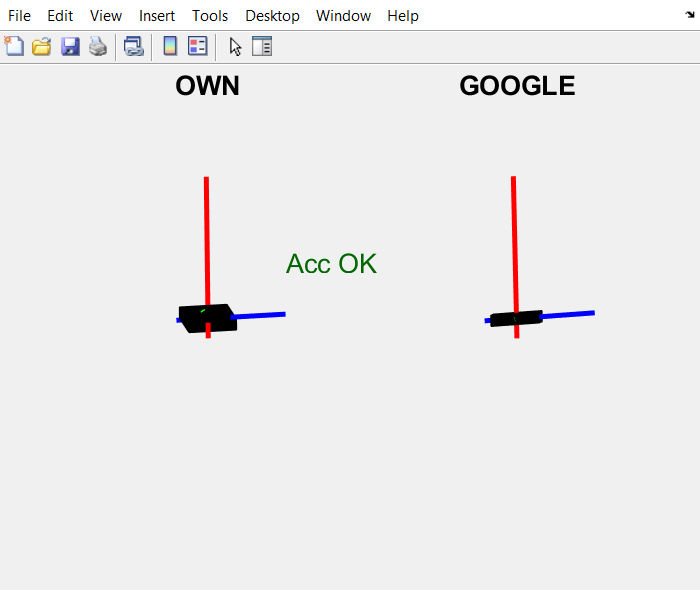
\includegraphics[width=0.6\textwidth]{images/maggentle.png}
 \caption{Gentle move and place it back to original place}
 \label{gentlemag}
\end{figure}

After I place the phone exactly beside my computer, the estimate picture of the phone starts to rotate.(For once)



\begin{figure}[H]
 \centering
 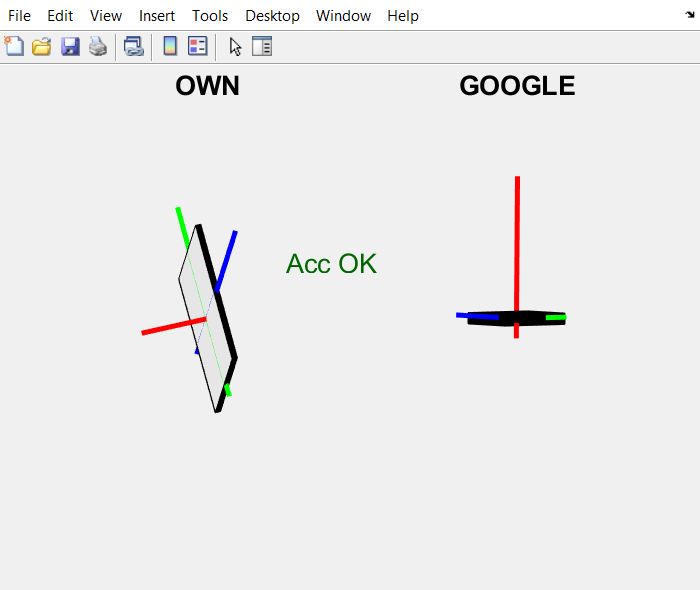
\includegraphics[width=0.6\textwidth]{images/rotatebesidecomputer.png}
 \caption{Place the phone beside computer}
 \label{rotatemag}
\end{figure}


When I try it later, the phone do not appear to rotate, but it stay at the wrong estimate posture which has a little offset from the estimation at the operating point. At this place with magnetic interference, both the estimation and the 'Google measurement' can neither return to the true result.

\begin{figure}[H]
 \centering
 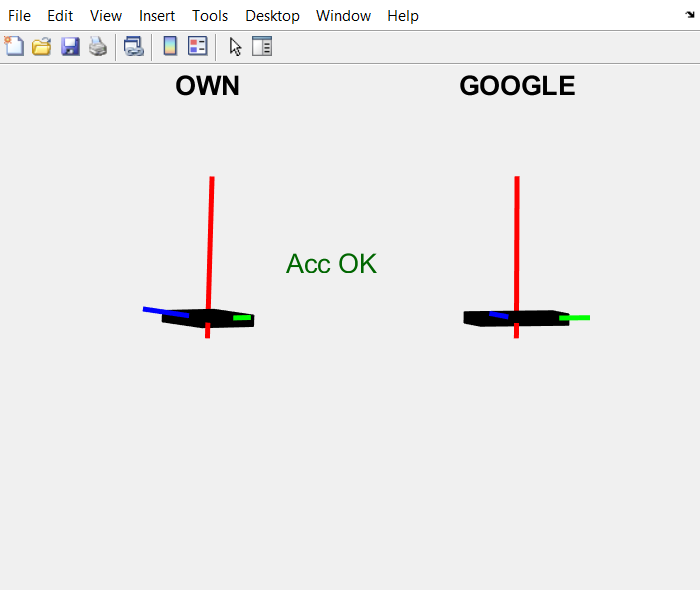
\includegraphics[width=0.6\textwidth]{images/biasmag.png}
 \caption{offset with interference }
 \label{offsetmag}
\end{figure}

When I try to return the phone to the operating point, I observed that our filter can return to the true state quicker than the Google measurement method, and nearly no bias from the beginning.

\begin{figure}[H]
 \centering
 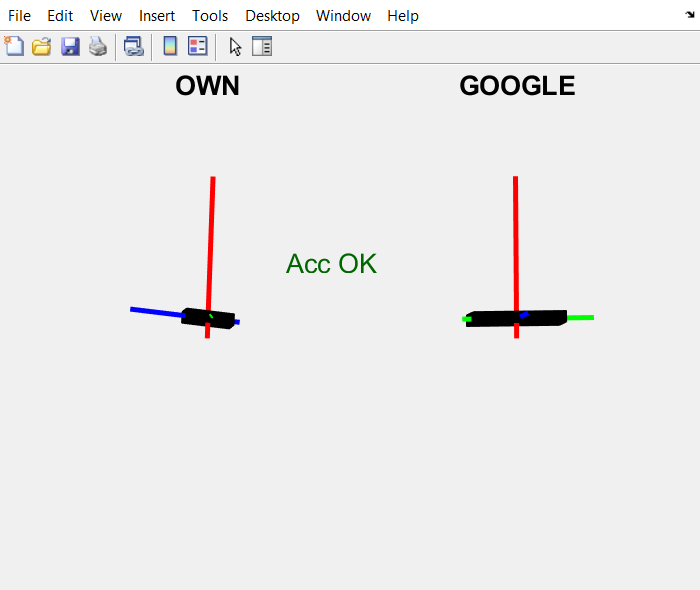
\includegraphics[width=0.6\textwidth]{images/returnmag.png}
 \caption{Return to beginning}
 \label{return}
\end{figure}

This says our filter now is kind of useable, at least with these three sensors we are allowed to get the true estimate using simplified model even suffering from interference.

\subsection{Task 11}

